\chapter{Ray Traced Soft Shadows}
Since rasterization didn't account the visibility of the pixel, we must look for other methods to handle shadows. Lots of shadow techniques have been proposed this years, for this article, we discuss the basic techniques and it's problems. At the end, we want to detail some techniques which is the future of shadow techniques, some accuracy, non-ad hoc, dynamic and artifact-free techniques. 

\section{Definitions}
By "Real-Time Shadows" \cite{b:rts}, a mathematical way to define a shadow in the context of computer graphics is to consider a point $\mathbf{p}$ in space. If each ray from the light source $\pounds$ reaches $\mathbf{p}$ without encountering any scene object (so-called \textit{blockers} or \textit{shadow casters}) on its way, $\mathbf{p}$ is considered \textit{lit}, otherwise in \textit{shadow}. The region of space where the light source is fully occluded is called \textit{umbra}, whereas the remaining shadow is referred to as \textit{penumbra}. The difference regions are depicted in figure \ref{f:shadow-definition}.

\begin{figure}\label{f:shadow-definition}
	\begin{center}
		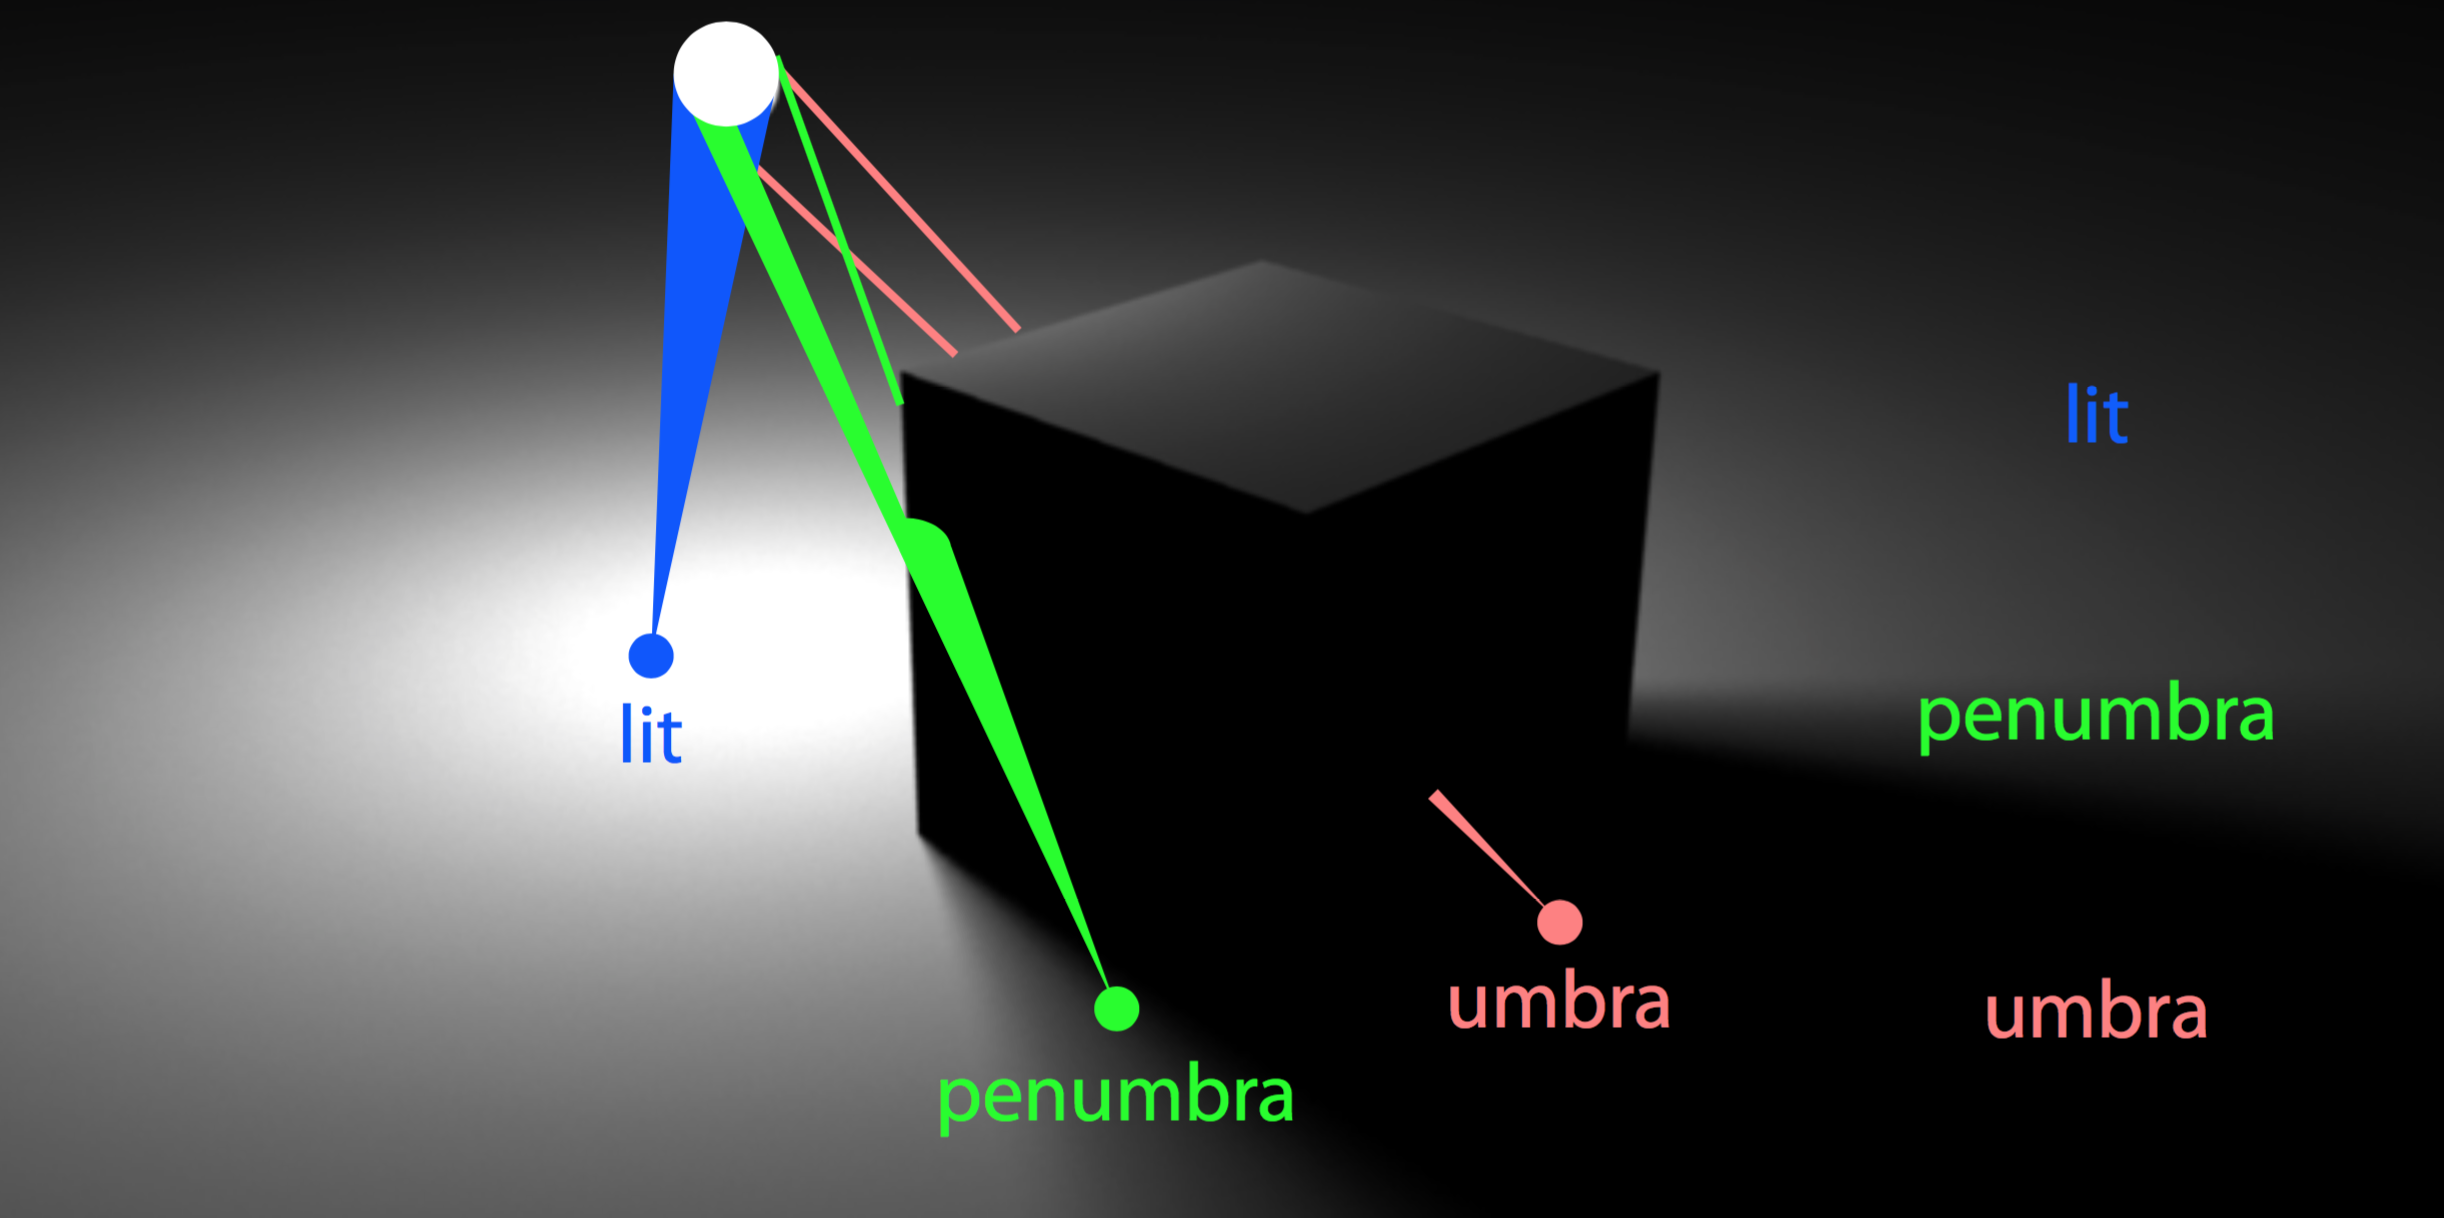
\includegraphics[width=1.0\textwidth]{graphics/shadows/shadow-definition}
	\end{center}
	\caption{Depending on the visibility of the source, there are three different regions in space; the umbra region, where the light is invisible, and the penumbra region, where it is partially visible constitute the shadow, the rest of the scene is lit(Images courtesy of "Real-Time Shadows").}
\end{figure}

For computing, the physical interaction can be described well by a \textit{soft shadow equation} that builds upon a modification of the \textit{rendering equation} introduced by Kajiya in 1986\cite{a:TheRenderingEquation} where we only consider direct light from the source:

\begin{equation}
	L_{o}(\mathbf{p},\omega)=\int_{\pounds}f_{r}(\mathbf{p},\omega,\mathbf{p}\rightarrow\mathbf{q})G(\mathbf{p},\mathbf{q})L_{e}(\mathbf{q},\mathbf{q}\rightarrow\mathbf{p})V(\mathbf{p},\mathbf{q})d\mathbf{q}
\end{equation}

where $L_{o}$ is the outgoing radiance in direction $\omega$ from point $\mathbf{p}$, $f$ is the BRDF (bidirectional reflectance function) encoding the material surface properties, $G$ is a geometric term taking the configuration of source and receiver into account, $L_{e}(\mathbf{q},\mathbf{q}\rightarrow\mathbf{p}$ is the emitted energy from the source point $\mathbf{q}$ towards $\mathbf{p}$, and finally $V(\mathbf{p},\mathbf{q})$ encodes the visibility and is zero if there is a blocker between the two points $\mathbf{q}$ and $\mathbf{p}$, and otherwise one.

It is very difficult to use this equation to compute shading and shadow. In practice we always make some assumptions to simplify this equation. Here two assumptions can be made:

\begin{itemize}
	\item The distance of the light to the receiver is relatively large (with respect to the light’s solid angle) and the light’s shape is simple, then the geometric term G varies little.
	\item The BRDF $f_{r}$ is mainly diffuse.
\end{itemize}

With these assumptions we can split the integral over the product of the two functions $G$ and $L_{e}$ into a product of integrals:

\begin{equation}
	L_{o}(\mathbf{p},\omega)=\underbrace{\int_{\pounds}f_{r}(\mathbf{p},\omega,\mathbf{p}\rightarrow\mathbf{q})G(\mathbf{p},\mathbf{q})d\mathbf{p}}_{\text{Shading}}\cdot\underbrace{\frac{1}{|\pounds|} \int_{\pounds} L_{e}(\mathbf{q},\mathbf{q}\rightarrow\mathbf{p})V(\mathbf{p},\mathbf{q})d\mathbf{q}}_{Shadow}
\end{equation} 
 
The simplification results in decoupling of shading and shadows.
Furthermore, we typically assume that the light source has homogeneous \textit{directional} radiation over its surface and is uniformly colored, causing $L_{e}$ to simplify to a constant $\bar{L}_{c}$. The equation can be wroten as:

\begin{equation}
	L_{o}(\mathbf{p},\omega)=\text{directIllum}(\mathbf{p},\omega,\pounds,\bar{L}_{c})\cdot V_{\pounds}(\mathbf{p})
\end{equation}

where $V_{\pounds}(\mathbf{p}$ is the \textit{visibility integral}

\begin{equation}
	V_{\pounds}(\mathbf{p}=\frac{1}{|\pounds|}\int_{\pounds}V(\mathbf{p},\mathbf{q})d\mathbf{q}
\end{equation}  

Based on these assumptions and approximations, we could separate shading and shadows from the rendering equation. So we can use rasterization to compute the color of a pixel without considering the shadows, while compute the shadow on somewhere else such as a shadow map by computing the visibility function only, then we blend them on the fragment shader. So in shadow technique, we mainly focus on visibility computation. 

But we should also remember, based on approximations, the results is not physically correct. If the light source has varied radiance density and color, and if the pixel is close to a large light source, etc, the wrongness might be perceived. But in most case in game, the results is convincing. 

\section{Basic Shadow Techniques}
There are four classes of shadow algorithms: \textit{projection shadows, shadow maps, shadow volumes} and \textit{ray tracing}. Projection shadow is limited to plane, and shadow volume is costly, so we only discuss shadow maps and ray tracing. we'll introduce shadow maps in this section and explain how ray tracing can solve the problems of which in the next sections.

\begin{figure}\label{f:shadow-maps}
	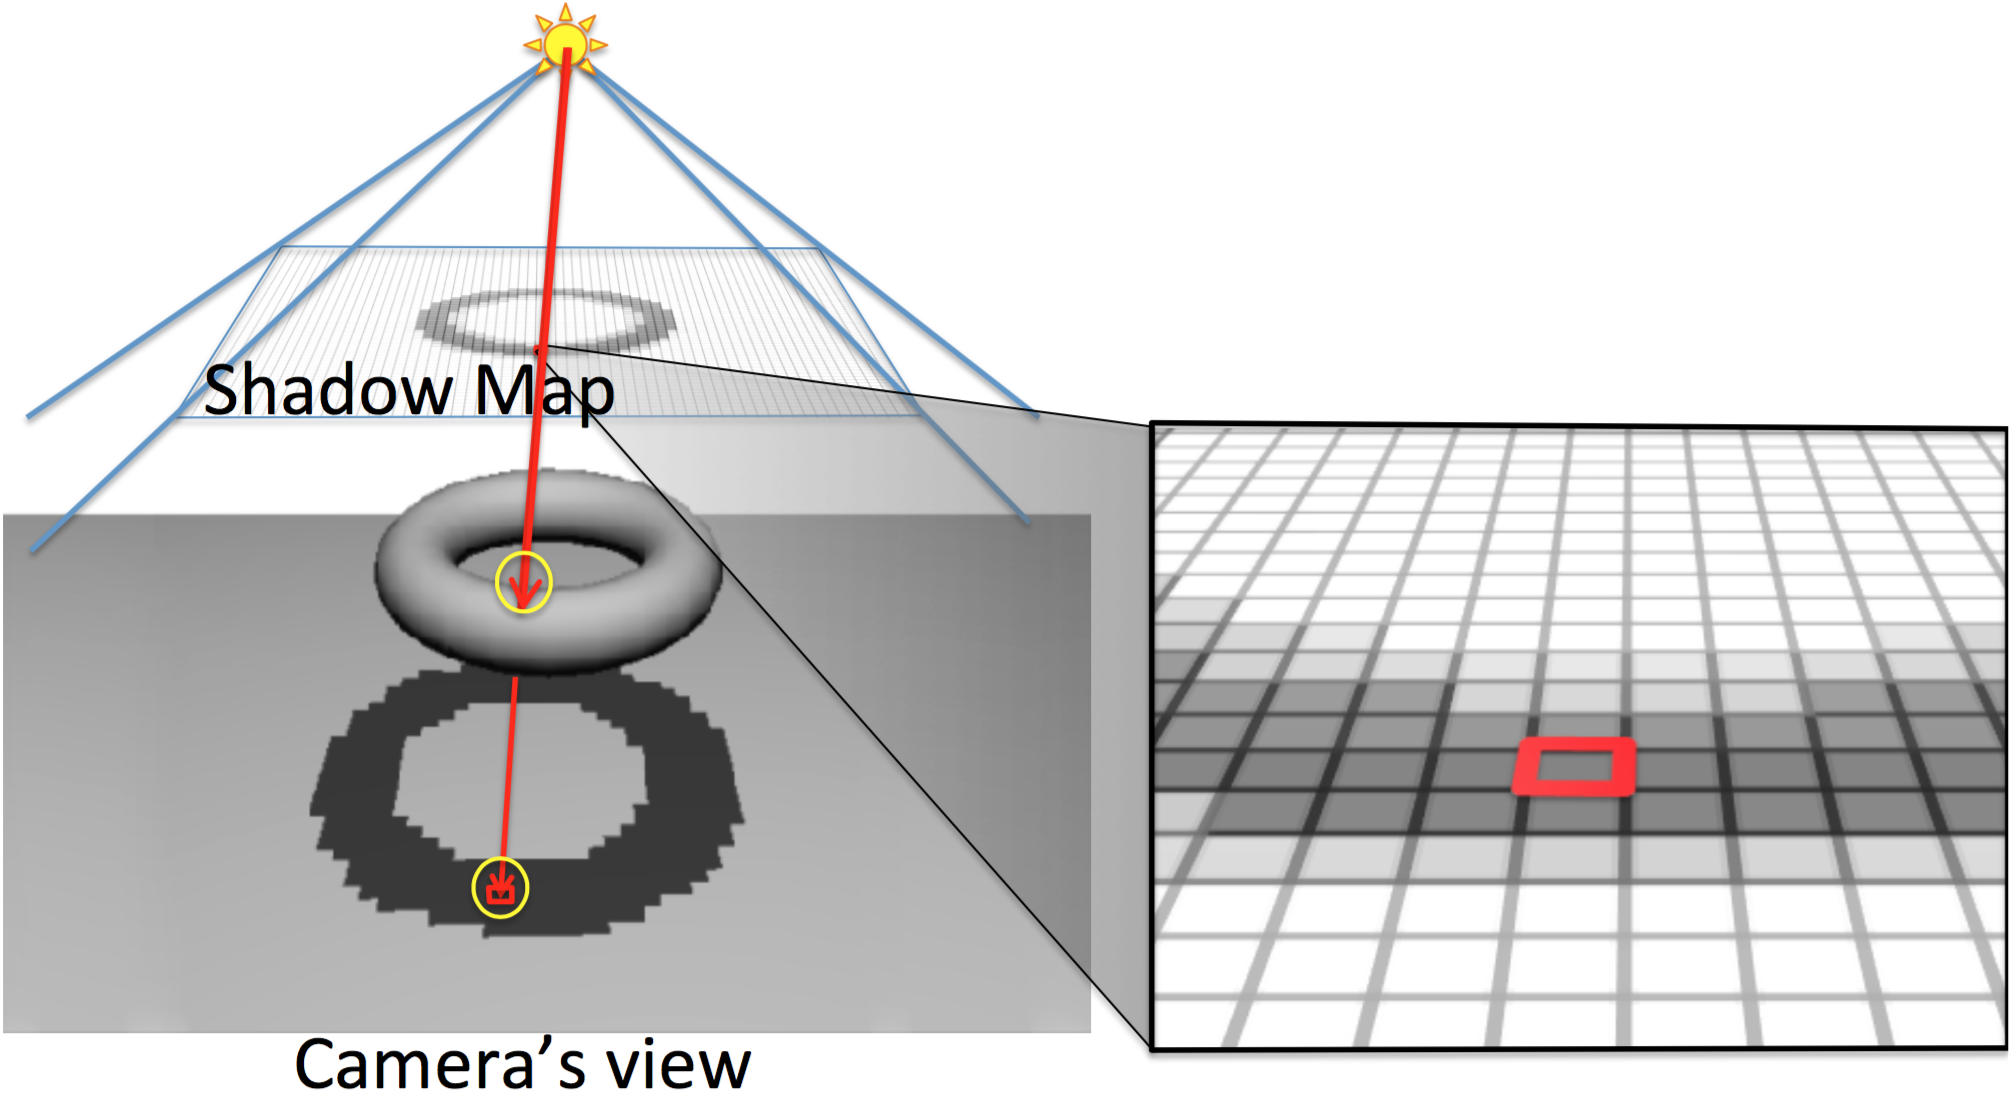
\includegraphics[width=1.0\textwidth]{graphics/shadows/shadow-map}
	\caption[][19mm]{Illustration of the shadow map algorithm.A fragment is in shadow if its depth is greater than the corresponding depth value in the shadow map(Images courtesy of "Real-Time Shadows").}
\end{figure}

We've already known for shadow computation, we only need take care about the visibility function. The shadow maps method was introduced by Williams in 1987\cite{a:Castingcurvedshadowsoncurvedsurfaces}. The algorithm starts by rendering an image from the light source and records the depth for each pixel. Next, the scene is rendered from the camera. For each pixel, the fragment shader tests if the sampled point's depth is greater than its depth in the light's view (in the shadow map). If so, the point is in shadow, else, the point is in lit.

Due to the discrete resolution of the shadow map, a view sample will rarely be the exactly represented in the shadow map. This results in two problems: \textit{perspective aliasing} and the need to introduce a tolerance threshold for comparison. The threshold, or \textit{bias}, must be fine tuned for each scene, and no bias is guaranteed to exist that avoids artifacts. A too large bias results in light leakage at contact shadows, while a too small bias results in incorrect self-shadowing. Increasing the shadow map resolution can be helpful, since then a smaller bias can be used. But it does not remove the problem.

To reduce perspective aliasing, the best way has been proven is cascaded shadow maps.


\section{Cascaded Shadow Maps}
The basic concept of cascaded shadow maps (CSMs) is easy to understand. Different areas of the camera frustum require shadow maps with different resolutions. Objects nearest the eye require a higher resolution than do more distant objects. The basic idea of CSMs is to partition the frustum into multiple frusta. A shadow map is rendered for each subfrustum; the pixel shader then samples from the map that most closely matches the required resolution, see figure \ref{f:cascaded-shadow-map}.

\begin{figure}
\sidecaption
	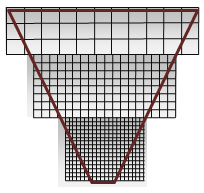
\includegraphics[width=0.65\textwidth]{graphics/shadows/cascaded-shadow-map}
	\caption{The shadow map with the most closely placed pixels (at the apex) is nearest the eye. Technically, these are maps of the same size. It shows good coverage—a 1:1 ratio for eye-space pixels and shadow-map texels.}
	\label{f:cascaded-shadow-map}
\end{figure}

CSMs require the following steps per fram:

\begin{enumerate}
	\item Partition the frustum into subfrusta.
	\item Compute an orthographic projection for each subfrustum.
	\item Render a shadow map for each subfrustum.
	\item Render the scene.
	\begin{enumerate}
		\item Bind the shadow maps and render.
		\item The vertex shader does the following:
		\begin{itemize}
			\item Computes texture coordinates for each light subfrustum (unless the needed texture coordinate is calculated in the pixel shader).
			\item Transforms and lights the vertex, and so on.
		\end{itemize}
		\item The pixel shader does the following:
		\begin{itemize}
			\item 	Determines the proper shadow map.
			\item Transforms the texture coordinates if necessary.
			\item Samples the cascade.
			\item Lights the pixel.
		\end{itemize}
	\end{enumerate}
\end{enumerate}

Since CSMs is dependent on the view position, it can not be precomputed. It is most used in the out door for sun light, which has a vast coverage. And it can generate dynamical shadow maps. For more details about CSMs please see \footnote{\url{https://msdn.microsoft.com/en-us/library/windows/desktop/ee416307(v=vs.85).aspx}}.

CSMs computation in real-time can be costly, in fact, when the eye moves very close to the geometry, the pixels nearest the eye can require so much resolution that even a $4096\times 4096$ shadow map is insufficient. Care must be taken, there are some good practices in Crytek\cite{a:PlayingwithReal-TimeShadows}, unlike the standard CSMs algorithm, which recompute the shadow cascades every frame, they update cost distributed across serval frames, see figure \ref{f:crytek-csm}.

\begin{figure*}\label{f:crytek-csm}
\begin{center}
	\begin{subfigure}[b]{0.442\textwidth}
		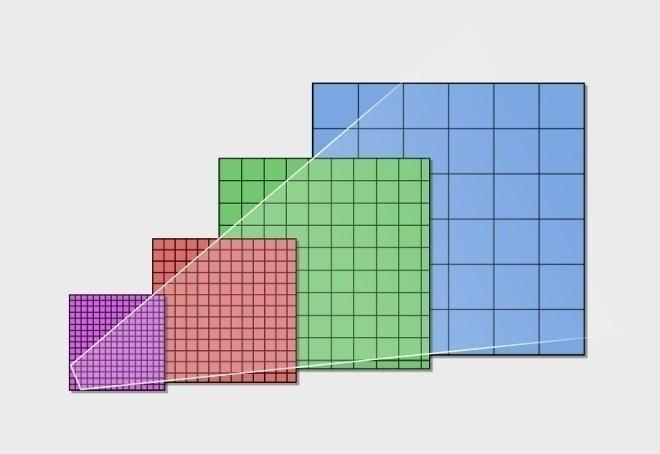
\includegraphics[width=1.0\textwidth]{graphics/shadows/crytek-csms-1}	
	\end{subfigure}
	\begin{subfigure}[b]{0.54\textwidth}
		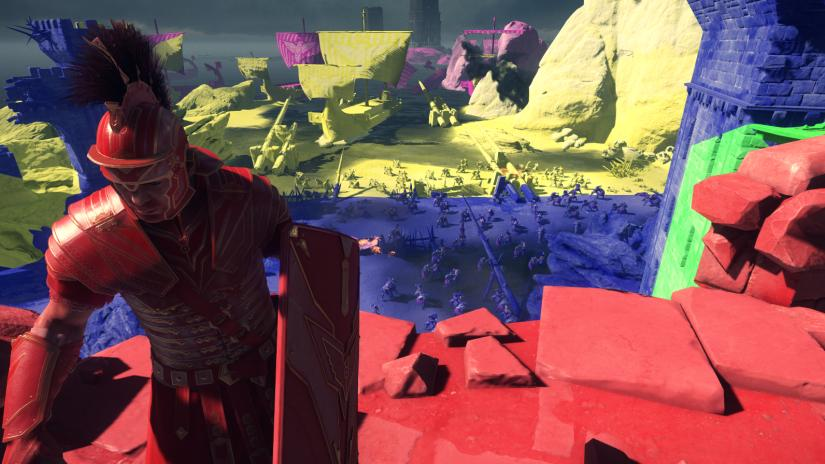
\includegraphics[width=1.0\textwidth]{graphics/shadows/crytek-csms-2}	
	\end{subfigure}
\end{center}
\caption{Crytek uses stencil buffer to tag the cascade volumes. The cascades will be cached and they updated cost distributed across serval frames.}
\end{figure*}

How does it works? They do this by using shadow cascades caching. Potential shadow-receiving areas are tagged in the stencil buffer by rendering frustum volumes, see \ref{f:crytek-csm}. In the next frame, the areas which is not covered by the CSMs will be computed. This allows to have a more sophisticated splitting into cascades, and shadow frustums adjusted to cover the camera view frustum conservatively.   

In this way, the cascades will overlap, in fragment shader, a cascade with a highest resolution in overlapping regions will be picked. Every frame, not all the cascades are updated, distance cascades are updated less frequently, cached shadow maps are not updated but are used for shadowing. Also you could find more knowledge about other shadow optimization in their presentation. 

Actually, this is a useful method in such situation that it needs to generate some view dependent data and submit them to the GPU dynamically. In such way, we could improve precision near the observer and to abstract information farther away, also, we update the farther data in less frequency. 


\section{Soft Shadow}
So far, we assume the light source is a single point. For any pixel, we only need to check if there is a occluder between the pixel and the light point. That make us can use a map to recompute this one-to-one check, which produce a \textit{hard shadow}. 

But real light source have a certain extent, it is not enough to just determine whether the light source is visible from a receiver point or not. Instead, the visible fraction of the light source has to be computed, which needs to cast lots of rays from the pixel to the light source area. 

There are mainly two group of approaches: one is images-based solution which typically resort to a standard shadow map, many of these methods use a simpler 2D filter to blur the edge; another one is geometry-based solution which avoid aliasing problems but comes along with a slower speed. You can get these knowledge from \cite{b:rts}. But here we only focus on ray traced soft shadow algorithms.

\begin{figure}\label{f:terms-of-soft-shadows}
\begin{center}
	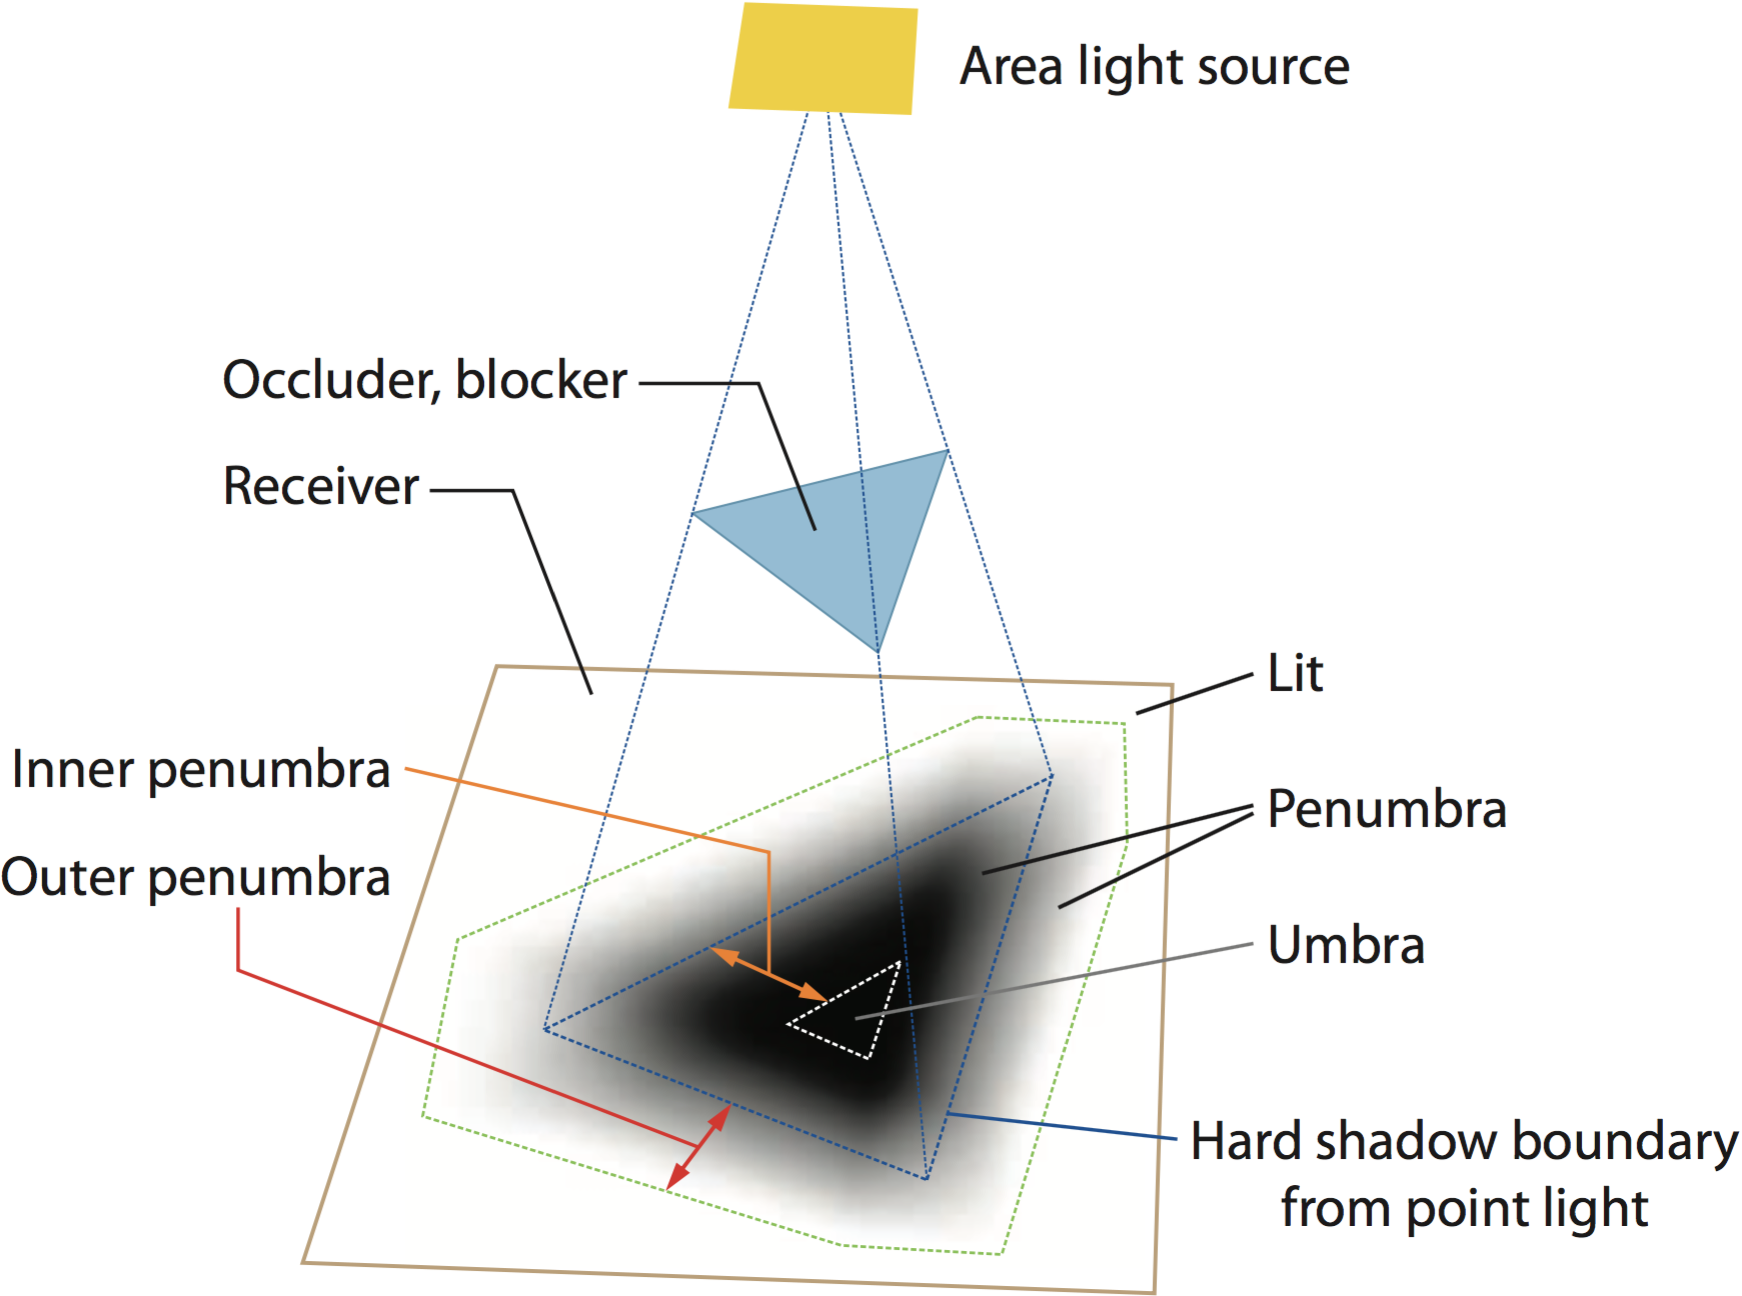
\includegraphics[width=0.7\textwidth]{graphics/shadows/soft-shadow-terms}
\end{center}
\caption[][30mm]{Terms of encountered when speaking of soft shadows(Images courtesy of "Real-Time Shadows").}
\end{figure}

With \textit{soft shadows} cast by extended light sources, three different kinds of illumination regions can be distinguished, see figure \ref{f:terms-of-soft-shadows}:

\begin{itemize}
	\item the \textit{umbra}, where the light source is completely occluded and which, hence, comprises scene points entirely in shadow;
	\item the \textit{lit region}, from which the light source is fully visible;
	\item the \textit{penumbra}, the intermediate transition region where the light is only partially occluded and, hence, still some partial illumination is received. 
\end{itemize}

\begin{figure}
\sidecaption
	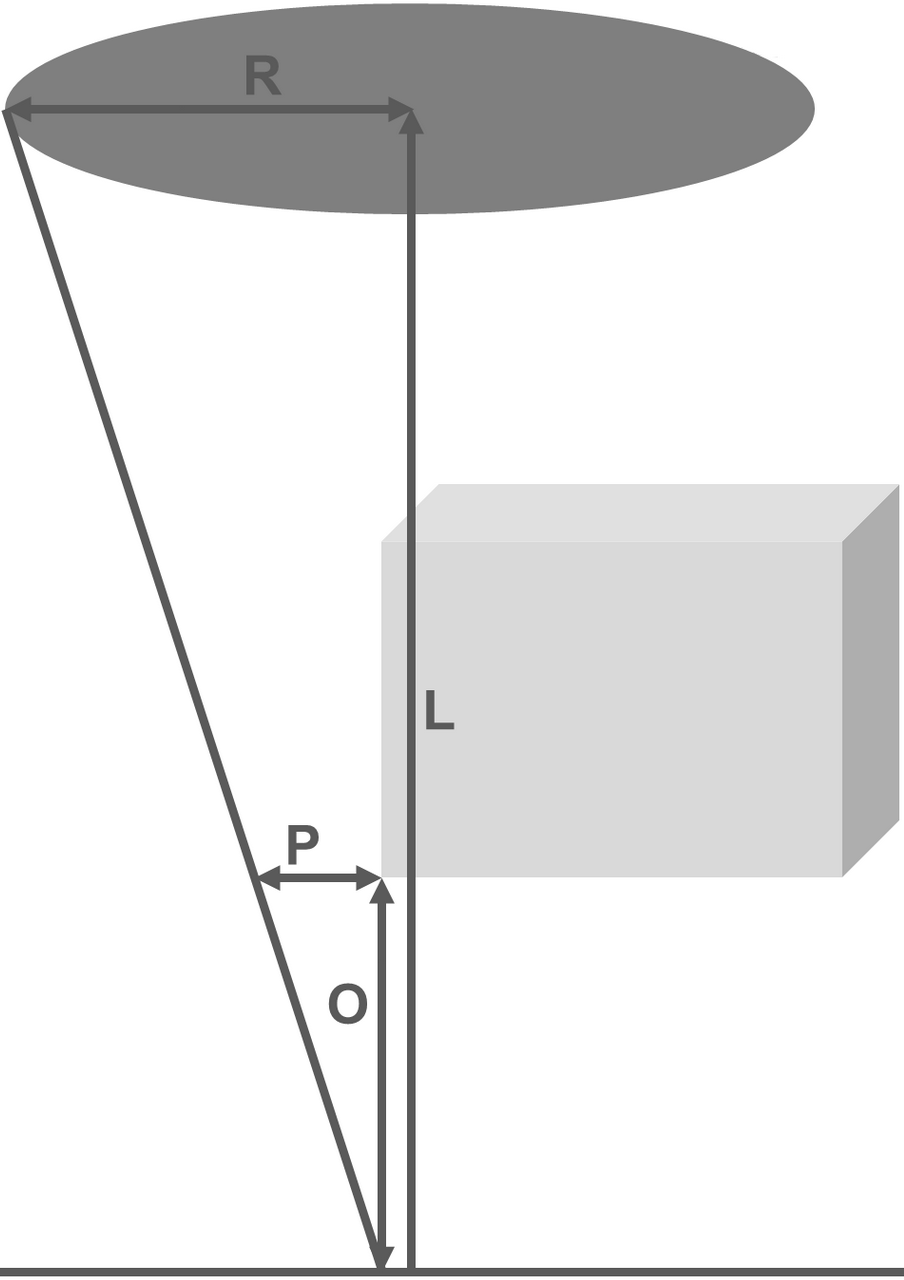
\includegraphics[width=0.65\textwidth]{graphics/shadows/penumbra-size-calculation}
	\caption{Analytically compute penumbra size}
	\label{f:penumbra-size-calculation}
\end{figure} 

It's hard to compute multi rays from pixel to light source areas in rendering time, in real time, we always like approximation. Typically we still treat the extended light as a single point light, and we can calculate the size of a penumbra based on three variables: the size of the light source $R$, the distance to the light source $L$, and the distance between the occluder and the surface on which the shadow is cast $O$. By moving the occluder closer to the surface, the penumbra is going to shrink, see figure \ref{f:penumbra-size-calculation}.


Based on these variables, we derive a simple formula for calculating the size of the penumbra $P$:

\begin{equation}
	P=\frac{RO}{L}
\end{equation}

By using ray tracing, it is easy to compute the distance from the pixel to the closet occluder. After we got this penumbra size, there are two methods we can use to approximate the soft shadows which we'll see in the next two sections. And most importantly, for every single pixel we just need one ray casting to achieve soft shadow accurately.



\section{Ray Traced Soft Shadows}
The first method we'll introduce comes from PowerVR ray tracing \footnote{\url{http://blog.imgtec.com/multimedia/implementing-fast-ray-traced-soft-shadows-in-a-game-engine}}. The PowerVR GR6500 and newer GPU include a \textit{PowerVR Ray Tracing Unit (RTU)}, which provides some graphics APIs for ray tracing your scene in GPU.

\begin{figure}\label{f:PowerVR-GPU-Architecture}
	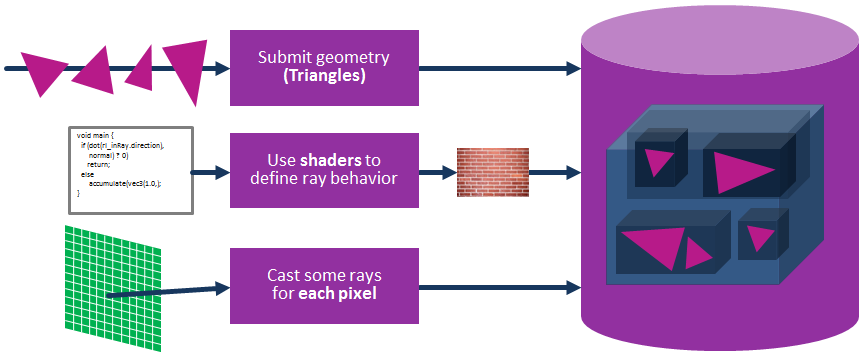
\includegraphics[width=1.0\textwidth]{graphics/shadows/Ray-tracing-in-games_Ray-tracing-inputs}
	\caption{Inputs to the ray tracer (world space scene intersection).}
\end{figure}

First, we need to submit the geometry to the ray tracer through a geometry pipeline similar to OpenGL and OpenGL ES. The ray tracer then takes this geometry and builds a 3D database of the scene. We only need to resubmit objects whose vertices have changed between consecutive frames, see figure \ref{f:PowerVR-GPU-Architecture}.

The ray tracer also requires a way to define the appearance of that geometry. In ray tracing, this is done by specifying what happens every time a ray collides with a triangle in your scene. A convenient way to describe this behaviour is using a shader. Just as a rasterizer converts a triangle into screen space to produce a fragment(i.e. you need a fragment shader to decide what color will be accumulated into the framebuffer for that fragment), a ray tracer will execute a ray shader every time a ray hits a triangle.

The final part of the process involves emitting some primary rays. For every pixel of the framebuffer, we need to define what primary rays are going to emitted for what pixel; this is done using a frame shader.

In their method, they handle soft shadow in deferred pass. It sends a ray from every pixel in the framebuffer to the light, and records the distance from the pixel to the closet occluder which form a distance buffer, see figure \ref{f:distance-buffer}.

\begin{figure}\label{f:distance-buffer}
	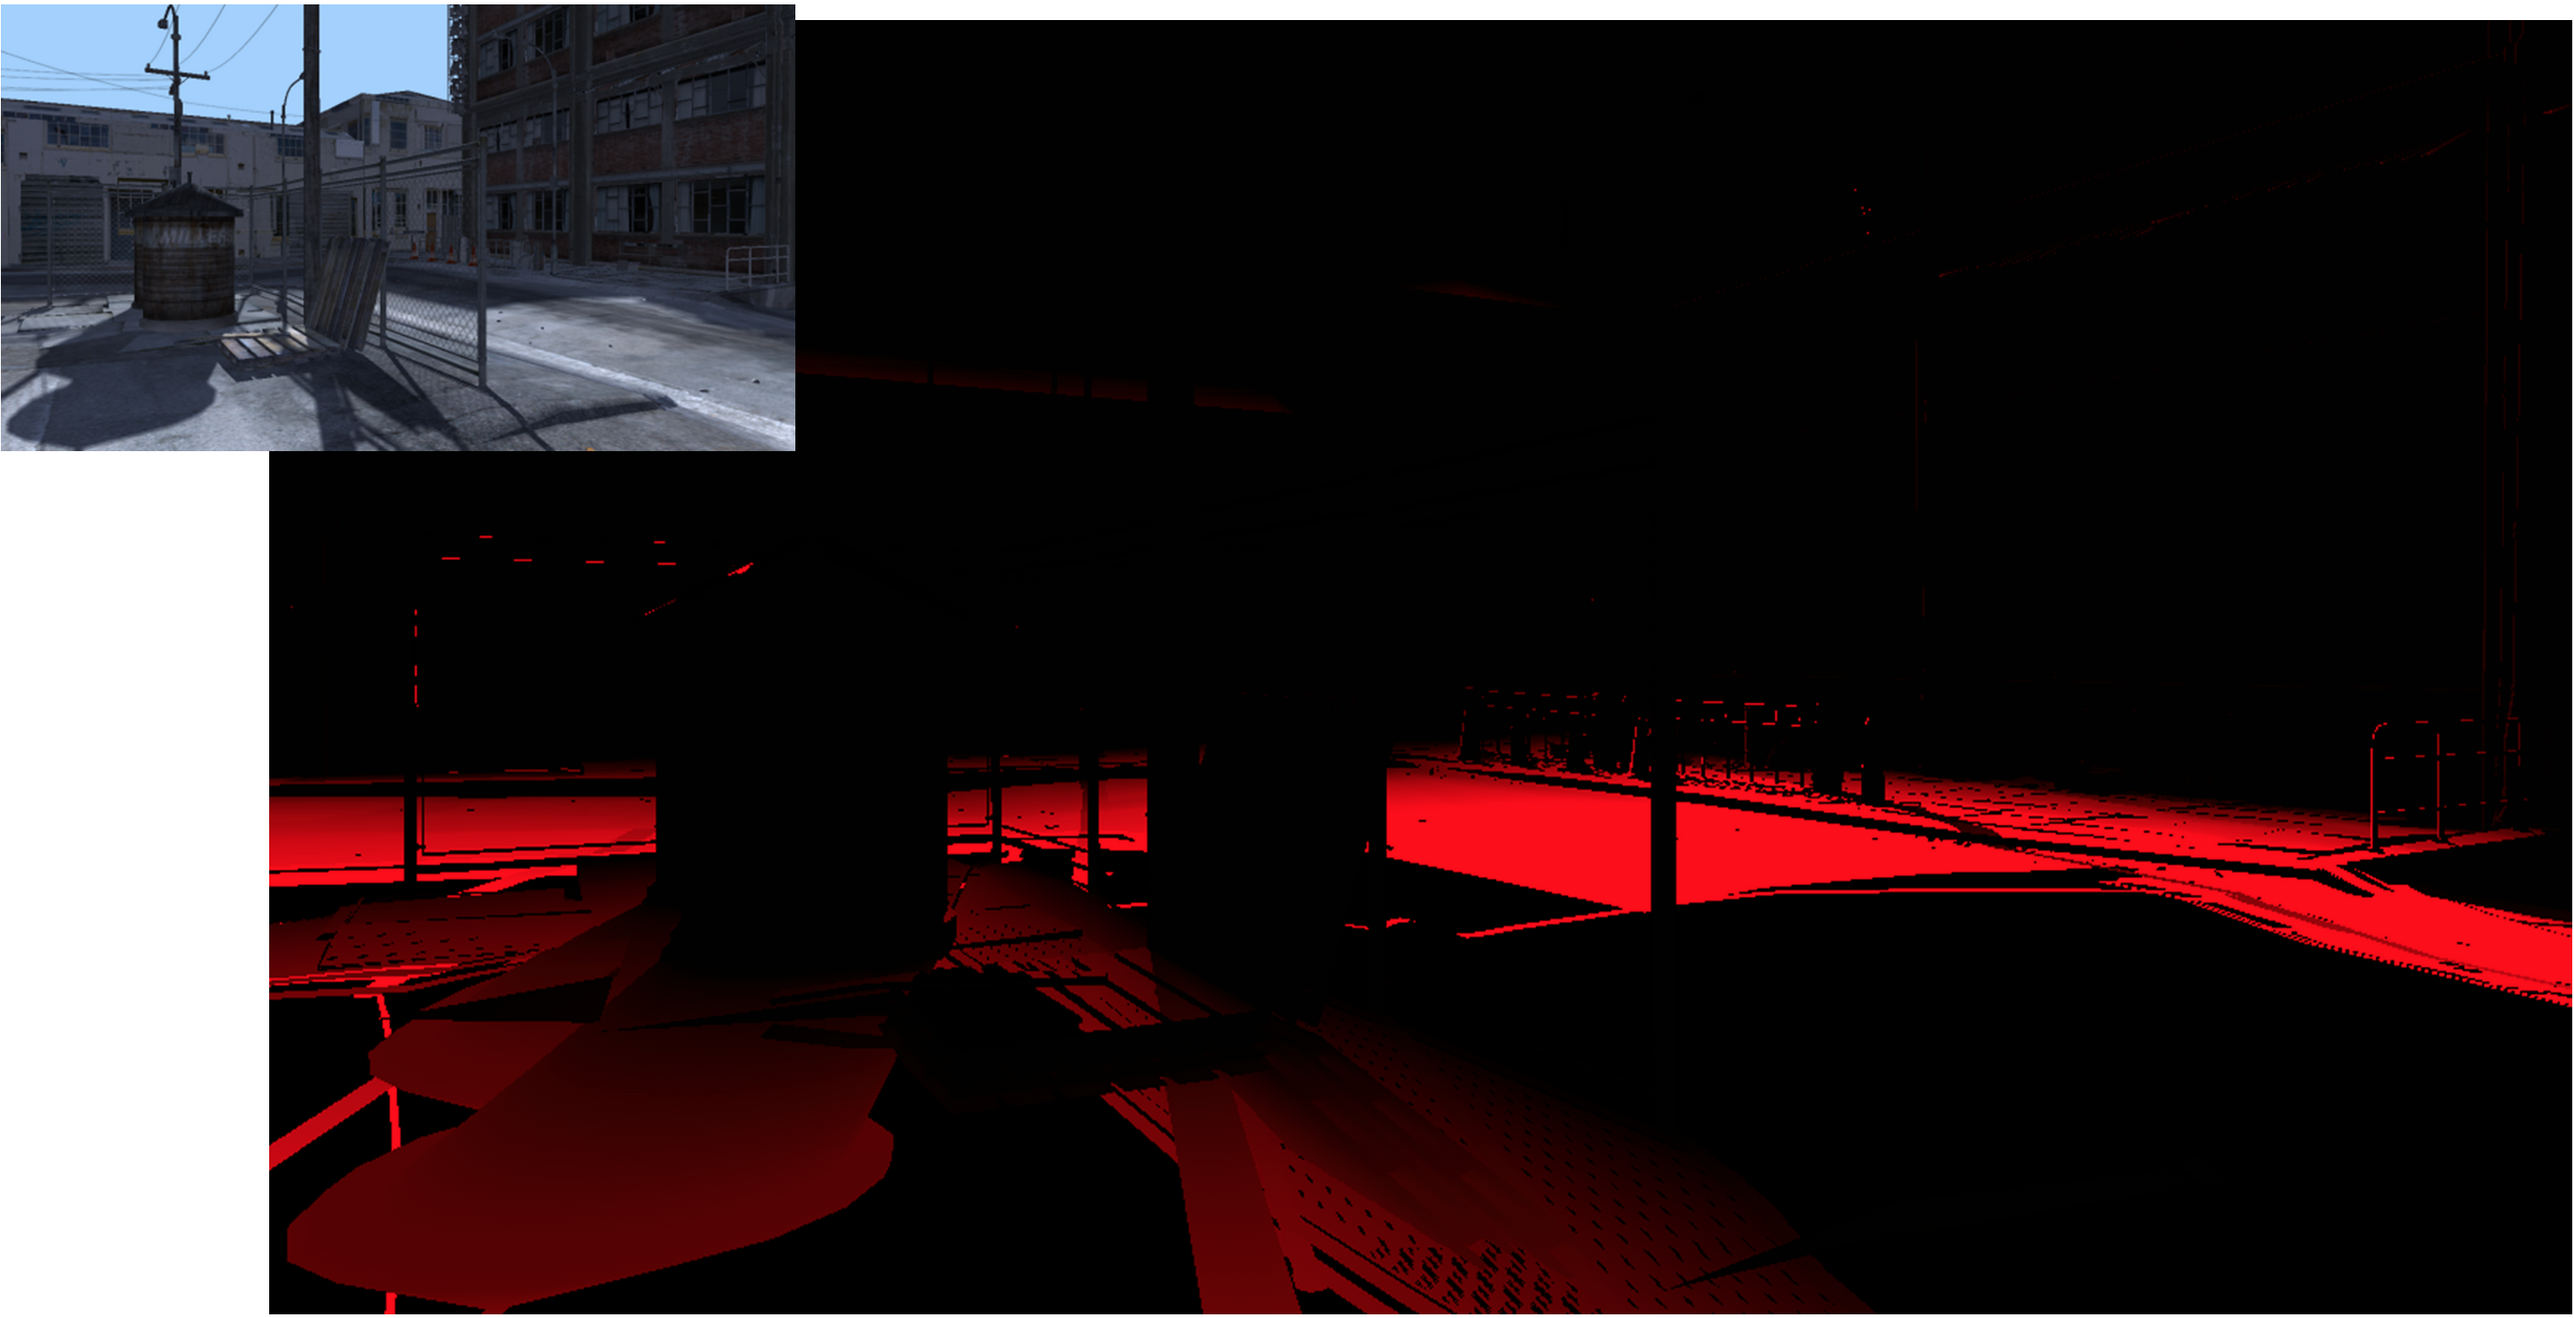
\includegraphics[width=1.0\textwidth]{graphics/shadows/ray-tracing-distance-buffer}
	\caption{Ray tracing distance buffer}
\end{figure}

As we get further away from the occluding objects, the value of the red component increases, representing a greater distance between the shadow pixel and the occluder.

Then they use a filter pass to calculate the shadow value for each pixel using this distance buffer.

\begin{figure}
\sidecaption
	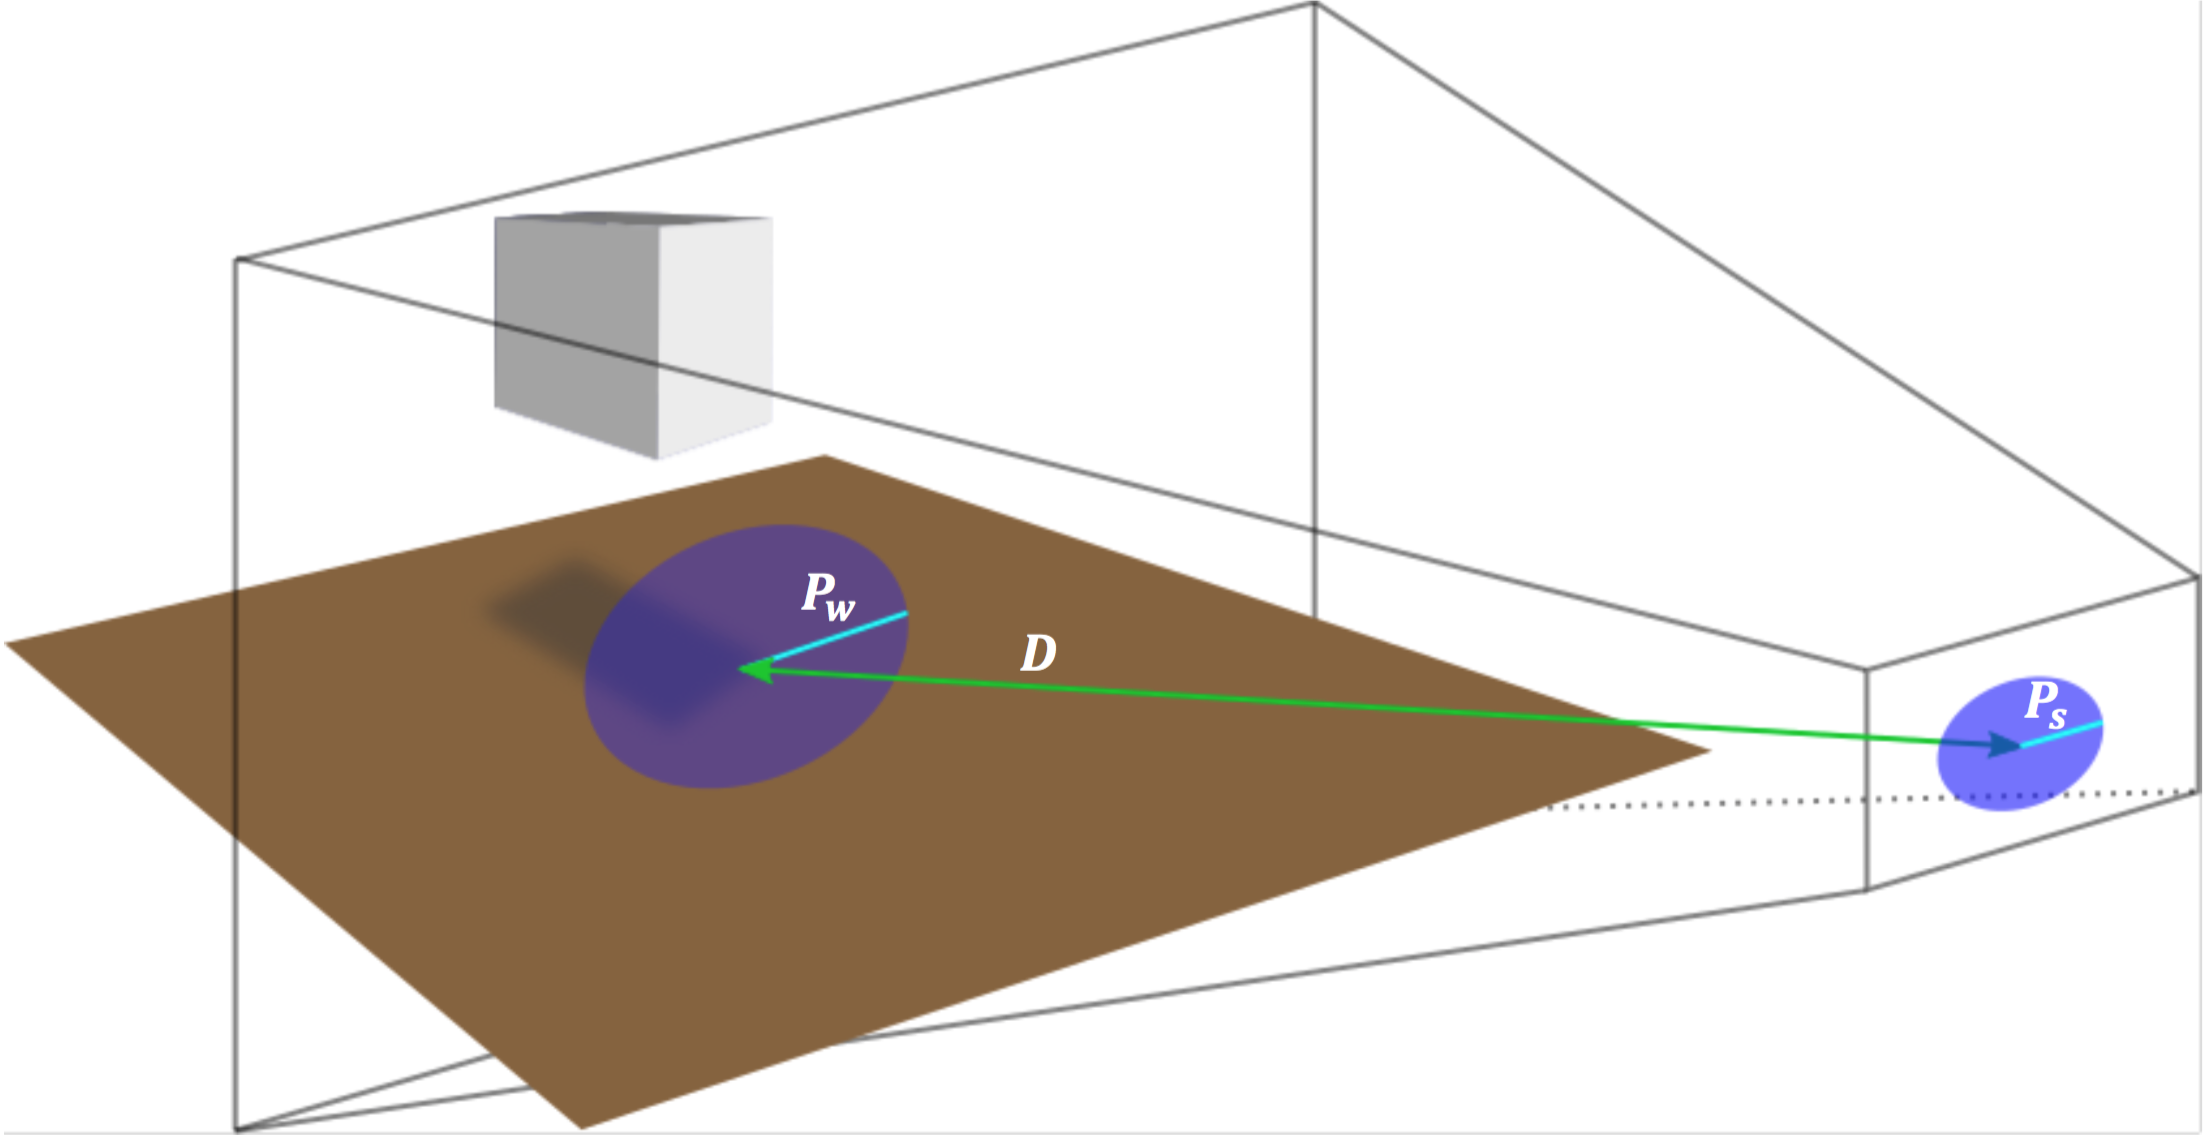
\includegraphics[width=0.65\textwidth]{graphics/shadows/kernel-width-section}
	\caption{Kernel width selection}
	\label{f:kernel-width-section}
\end{figure}

For every pixel, they use this distance to calculate the penumbra size and use this penumbra to choose a blur kernel radius: just project the penumbra width from world space into screen space and the with in the screen space is the kernel width, see figure \ref{f:kernel-width-section}.

The distance selection is different according to whether the pixel is in shadow or not, see figure \ref{f:distance-selection}. If the pixel is in shadow, it's sample, the value of the  distance buffer is the penumbra size; When the pixel is lit, they use a cross search algorithm to locate another pixel with a ray that contributes to the penumbra. If any pixels on the X or Y axis that are in shadow (i.e. have valid distance values) are found, they'll pick the maximum distance to occluder value and use it to calculate the penumbra region for this pixel; 

\begin{figure}\label{f:distance-selection}
\begin{center}
	\begin{subfigure}[b]{0.45\textwidth}
		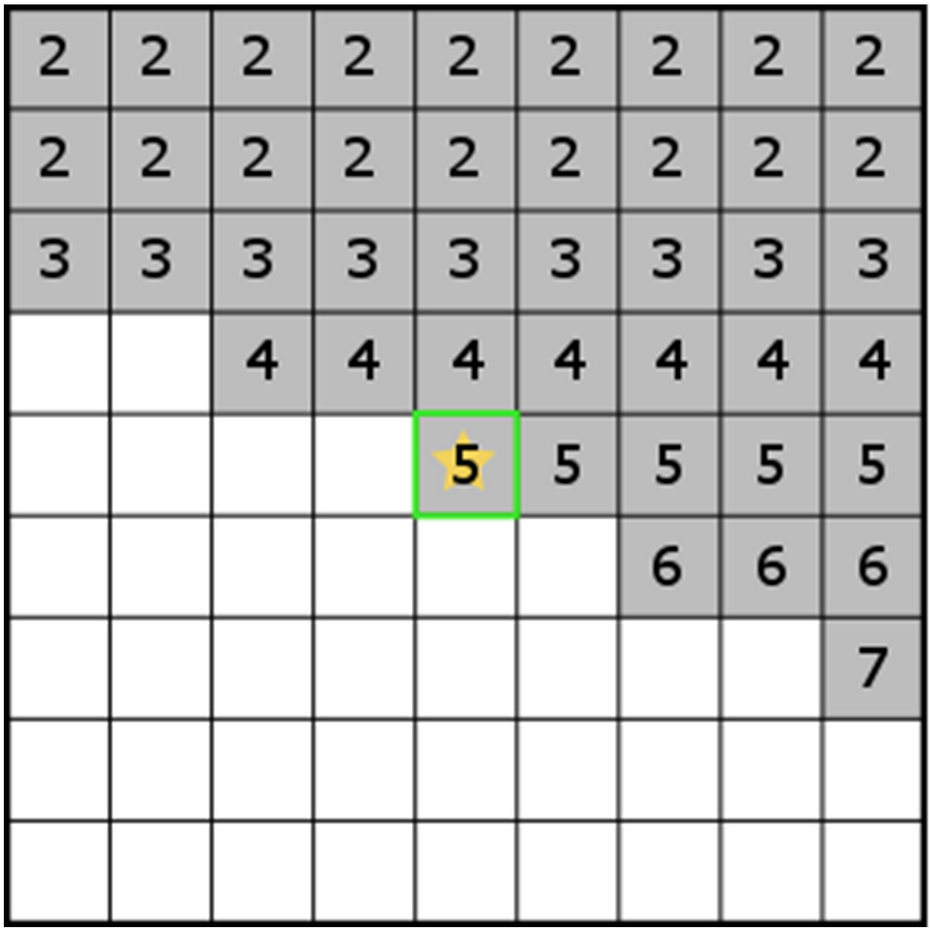
\includegraphics[width=1.0\textwidth]{graphics/shadows/penumbra-size-calculation-1}	
		\caption{in shadow}
	\end{subfigure}
	\begin{subfigure}[b]{0.45\textwidth}
		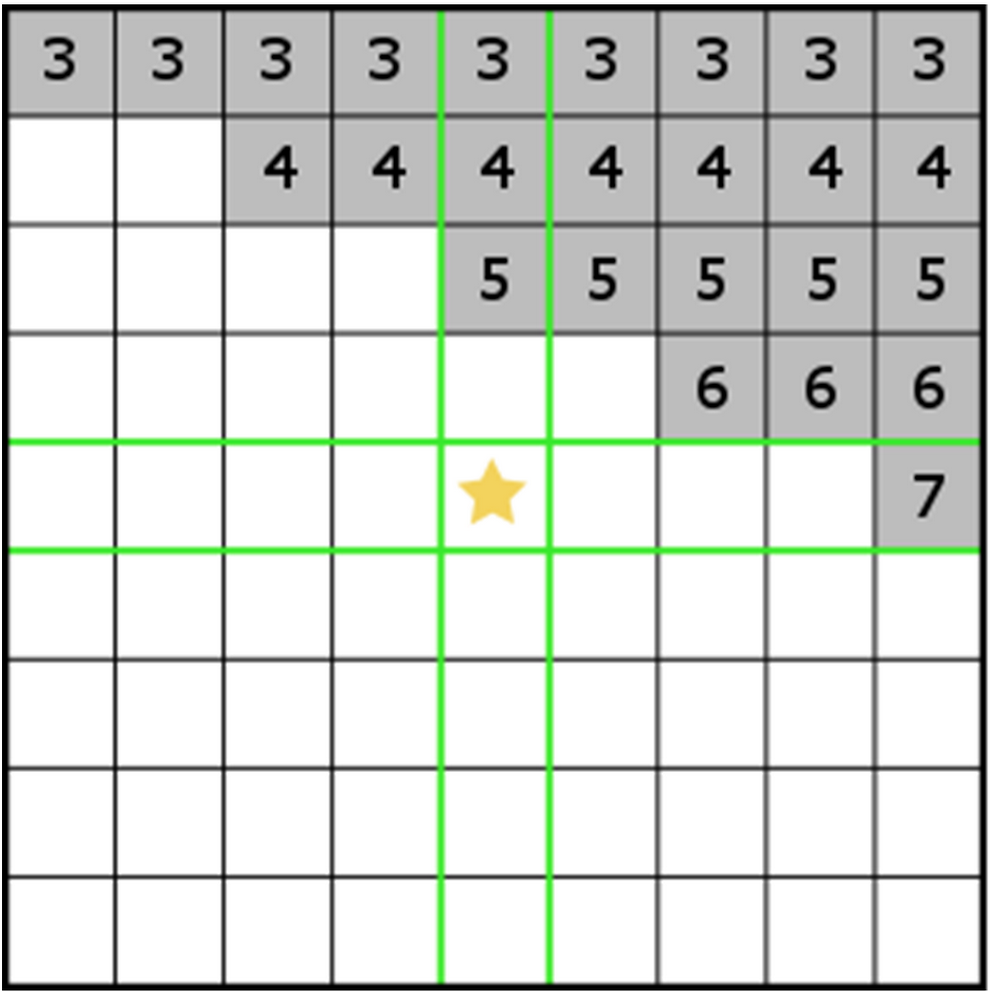
\includegraphics[width=1.0\textwidth]{graphics/shadows/penumbra-size-calculation-2}	
		\caption{not in shadow}
	\end{subfigure}
\end{center}
\caption{Penumbra size calculation.}
\end{figure}




\section{Ray Traced Distance Field Soft Shadows}
In Unreal Engine 4, they use distance field to represent the whole scene in GPU, so they can use a sphere tracing to compute the penumbra size.

\begin{figure}
	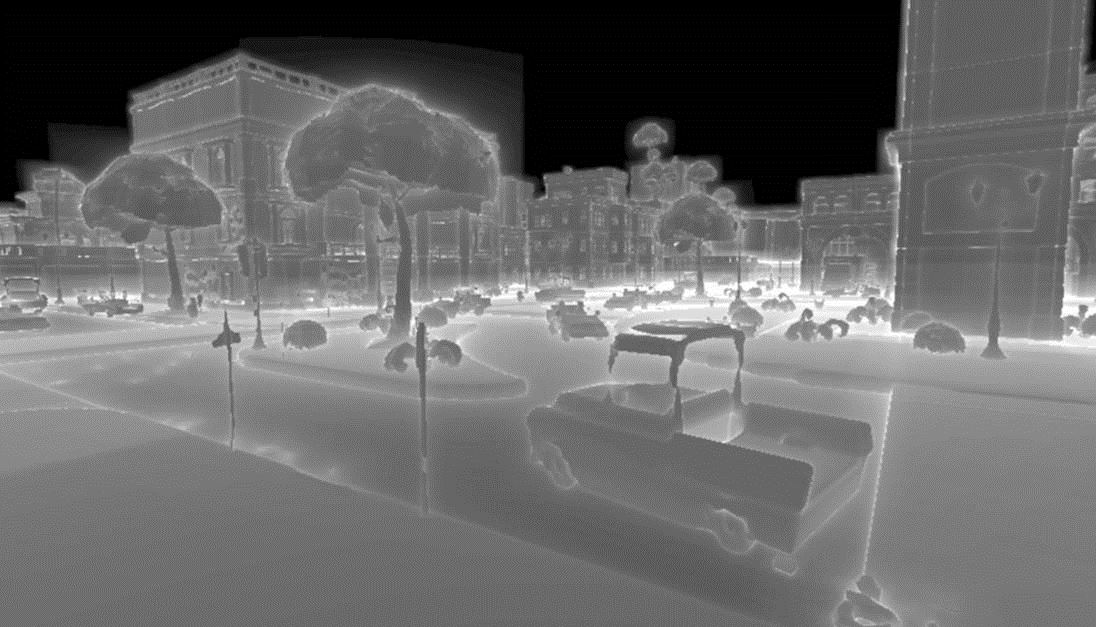
\includegraphics[width=1.0\textwidth]{graphics/shadows/VisualizeMeshDistanceFields}
	\caption{In Unreal Engine 4, every mesh can generate a distance field which will be submitted to GPU and be used. So they can do fast sphere tracing in GPU.}
\end{figure}

By using distance fields, it is easy to get an approximate cone intersection with no extra cost: in every step, record the distance to the closet surface and find the minimum distance in all steps, see figure \ref{f:ConeTrace}. This makes it possible to do very soft area shadows by ray tracing distance fields. This property is also key to Distance Field AO as a small number of cones can compute a soft visibility for the entire hemisphere of a receiver point.

\begin{figure}
\sidecaption
	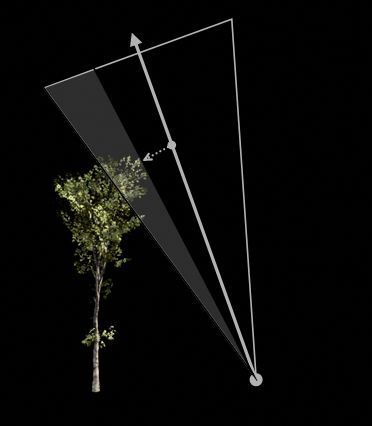
\includegraphics[width=0.65\textwidth]{graphics/shadows/ConeTrace}
	\caption{Hello}
	\label{f:ConeTrace}
\end{figure}


To calculate shadowing, a ray is traced from the point being shaded through the scene's signed distance fields toward each light. The closet distance to an occluder is used to approximate a cone trace for about the same cost as the ray trace.

After the cone tracing, they use a approximation to compute the visibility directly:

\begin{equation}
	\text{Shadow}=1-Min(\frac{\text{Distance to Surface}}{\text{Cone Radius}})
\end{equation}

Cone radius is determined by the property 'Source Radius' of a point light and 'Light Source Angle' of a directional light. This approximation works surprisingly well. But unfortunately, it only accounts the outer penumbra.

\begin{figure}\label{f:soft-shadow-ue4}
	\includegraphics[width=1.0\textwidth]{graphics/shadows/soft-shadow-ue4}
	\caption{In Unreal Engine 4, they use CSMs to shadow the nearest areas and use SDF traced shadows to shadow the further regions}
\end{figure}

One shortage using distance field is that the vertex animation, like foliages, can not be represented. In Unreal Engine 4, for directional lights, they use cascaded shadow maps for the near noticeable areas which can handle the animated foliages, and use signed distance field ray traced shadows for the distance areas, see figure \ref{f:soft-shadow-ue4}.


\section{Conclusions}
In this section, we mainly discussed ray traced soft shadow. The ray tracing calculation can resort either a hardware ray tracer (e.g, PowerVR ray tracing) or a distance field scene representation in GPU. They both use a single ray to approximate the soft shadow, so it is very efficient. 

We discussed two different algorithms which using ray tracing to compute soft shadow. One use the distance to the closet occluder to compute the penumbra size, then use the penumbra size to choose a blur kernel width adaptively, which is used in a filter pass. Another one is use the distance to the occluder approximate the visibility directly.

The difference also comes from the truth that they have a different ray tracing architecture. In PowerVR ray tracing, the ray tracing part is a middleware, for utilizing the multi GPU cores, the ray tracing process is like the traditional rasterization process, we use a ray trace shader to accumulate the result to a framebuffer, in this shadow algorithm is a distance buffer. So we can not fetch the ray tracing result directly, but we can do this in Unreal Engine 4, since they implement the ray tracing themselves by a fragment shader.

We also detailed cascaded shadow maps technique because it is the most important shadow technique, and we want to show the performance and advantages of ray traced shadow by comparing it to CSMs.

This ray traced shadow has several advantages over cascaded shadow maps or other common techniques:

\begin{itemize}
	\item There are no shadow map resolution issues since it is all based in screen space
	\item There are no banding, noise or buzzing effects due to sampling errors
	\item There are no biasing problems (sometimes called Peter-Panning) since you are shooting rays directly off geometry and therefore getting perfect contact between the shadow and the casting object
\end{itemize}


Furthermore, in PowerVR ray tracing, using the hardware based technique reduces memory traffic compared with cascaded shadows. In one test, a single scene used up 233MB of memory for cascaded shadows compared with 164MB for ray tracing. Subtract the “G Buffer” setup cost of the scene and ray tracing can result in a 50 percent reduction in memory traffic. 

In Unreal Engine 4, it is said to be 30-50\% faster than traditional shadowmaps (cubemap/CSMs).